%%
%% Copyright 2007-2018 Elsevier Ltd
%% 
%% This file is part of the 'Elsarticle Bundle'.
%% ---------------------------------------------
%% 
%% It may be distributed under the conditions of the LaTeX P{sec:betweenness}
%% License, either version 1.2 of this license or (at your option) any
%% later version.  The latest version of this license is in
%%    http://www.latex-project.org/lppl.txt
%% and version 1.2 or later is part of all distributions of LaTeX
%% version 1999/12/01 or later.
%% 
%% The list of all files belonging to the 'Elsarticle Bundle' is
%% given in the file `manifest.txt'.
%% 
%% Template article for Elsevier's document class `elsarticle'
%% with harvard style bibliographic references

\documentclass[preprint,12pt,authoryear]{elsarticle}

%% Use the option review to obtain double line spacing
%% \documentclass[authoryear,preprint,review,12pt]{elsarticle}

%% Use the options 1p,twocolumn; 3p; 3p,twocolumn; 5p; or 5p,twocolumn
%% for a journal layout:
%% \documentclass[final,1p,times,authoryear]{elsarticle}
%% \documentclass[final,1p,times,twocolumn,authoryear]{elsarticle}
%% \documentclass[final,3p,times,authoryear]{elsarticle}
%% \documentclass[final,3p,times,twocolumn,authoryear]{elsarticle}
%% \documentclass[final,5p,times,authoryear]{elsarticle}
%% \documentclass[final,5p,times,twocolumn,authoryear]{elsarticle}

%% For including figures, graphicx.sty has been loaded in
%% elsarticle.cls. If you prefer to use the old commands
%% please give \usepackage{epsfig}

%% The amssymb package provides various useful mathematical symbols
\usepackage{amssymb}

\usepackage{float}%exact location
\usepackage{graphicx}
\usepackage{caption}
\usepackage{subcaption}

\usepackage{hhline}
\usepackage{multirow}
\usepackage[utf8]{inputenc}
\usepackage[T1]{fontenc}
\usepackage{lmodern}
\usepackage{epsfig}
\usepackage{amsthm}
\usepackage{array}
\usepackage{algorithmicx}
\usepackage[ruled]{algorithm}
\usepackage{algpseudocode, caption}
 
\usepackage[cmex10]{amsmath}
%% The amsthm package provides extended theorem environments
%% \usepackage{amsthm}

%% The lineno packages adds line numbers. Start line numbering with
%% \begin{linenumbers}, end it with \end{linenumbers}. Or switch it on
%% for the whole article with \linenumbers.
%% \usepackage{lineno}

\newcommand{\D}[3]{\delta_{{#1}{#2}}({#3})}
\newcommand{\V}[2]{V_{#2}({#1})}
\newcommand{\LV}[2]{V_{\le #2}({#1})}
\newcommand{\E}[2]{E_{#2}({#1})}
\newcommand{\LE}[2]{E_{\le #2}({#1})}
\newcommand{\EH}[3]{E_{{\le #2}:{\le #3}}({#1})}

\newcommand{\EN}[1]{\mathcal{E}_{{#1}}}
\newcommand{\ENN}[2]{\mathcal{E}_{{#1}}^{{#2}}}
\newcommand{\FNN}[2]{\mathcal{F}_{{#1}}^{{#2}}}
\newcommand{\XN}[1]{\mathcal{X}_{{#1}}}
\newcommand{\CC}[1]{\mathcal{C}_{{#1}}}

\newcommand{\B}[1]{B({#1})}
\newcommand{\BE}[1]{B^{\mathcal{E}}({#1})}
\newcommand{\BX}[1]{B^{\mathcal{X}}({#1})}

\newcommand{\NX}{n_{x}}
\newcommand{\MX}{m_{x}}
\newcommand{\NE}{n_{e}}
\newcommand{\ME}{m_{e}}
\newcommand{\NC}{n_{c}}
\newcommand{\MC}{m_{c}}

\theoremstyle{definition}
\newtheorem{definition}{Definition}[section]

\newtheorem{theorem}{Theorem}[section]
\newtheorem{example}[theorem]{Example}

\journal{Social Networks}

\begin{document}

\begin{frontmatter}

%% Title, authors and addresses

%% use the tnoteref command within \title for footnotes;
%% use the tnotetext command for theassociated footnote;
%% use the fnref command within \author or \address for footnotes;
%% use the fntext command for theassociated footnote;
%% use the corref command within \author for corresponding author footnotes;
%% use the cortext command for theassociated footnote;
%% use the ead command for the email address,
%% and the form \ead[url] for the home page:
%% \title{Title\tnoteref{label1}}
%% \tnotetext[label1]{}
%% \author{Name\corref{cor1}\fnref{label2}}
%% \ead{email address}
%% \ead[url]{home page}
%% \fntext[label2]{}
%% \cortext[cor1]{}
%% \address{Address\fnref{label3}}
%% \fntext[label3]{}

\title{Multi-order Friendship Network Betweenness}

%% use optional labels to link authors explicitly to addresses:
%% \author[label1,label2]{}
%% \address[label1]{}
%% \address[label2]{}

\author{}

\address{}

\begin{abstract}
In this section, we define terms that represent two types of ego networks, ego networks and multi-layered ego networks (Section~\ref{x-ego_definition}), as well as the betweenness of a vertex in its ego and x-ego networks (Section~\ref{sec:betweenness}).
We then present several properties of the multi-layered ego networks (Section~\ref{x-go_properties}).
Our betweenness computation algorithm in Section~\ref{computation} takes advantage of these properties.


\end{abstract}

\begin{keyword}
Ego Networks \sep Betweenness Centrality
%% keywords here, in the form: keyword \sep keyword

%% PACS codes here, in the form: \PACS code \sep code

%% MSC codes here, in the form: \MSC code \sep code
%% or \MSC[2008] code \sep code (2000 is the default)

\end{keyword}

\end{frontmatter}

%% \linenumbers

%% main text
\section{Introduction}\label{sec:introduction}
In this section, we define terms that represent two types of ego networks, ego networks and multi-layered ego networks (Section~\ref{x-ego_definition}), as well as the betweenness of a vertex in its ego and x-ego networks (Section~\ref{sec:betweenness}).
We then present several properties of the multi-layered ego networks (Section~\ref{x-go_properties}).
Our betweenness computation algorithm in Section~\ref{computation} takes advantage of these properties.

An ego network (also called egocentric network) consists of the alters connected to ego, along with the links between
ego and alters, and links among alters (\cite{ego:2018}).

\section{Multi-order Friendship Networks}\label{sec:multi-order-friendship-network}
\begin{table}[t]
\captionsetup[subfigure]{aboveskip=-2pt, belowskip=-1pt}
\center
\caption{Summary of notation}\label{table:symbols}
\small
    \begin{tabular}{| p{1.2cm} | p{10cm} |}
        \hline
        Symbol & Description \\
        \hline
        \hline
        $\V{v}{i}$ & set of $i$-hop neighbors of vertex $v$ ($\V{v}{0} = \{ v \}$)\\
        $\LV{v}{i}$ & set of vertices that are at most $i$ hops away from vertex $v$ (i.e., $\LV{v}{i} = \cup_{k = 0}^{i} \V{v}{k}) $\\
        $\E{v}{i}$ & set of edges connecting two vertices in $\V{v}{i}$ ($\E{v}{0}$=$\emptyset$)\\
        $\LE{v}{i}$ & set of edges connecting two vertices in $\LV{v}{i}$\\
        \hline
    \end{tabular}
\end{table}
In this section, we formally define {\it multi-order egocentric friendship networks}, while we also introduce {\it multi-order egocentric networks} formally, and then provide the definition of betweenness centrality over such networks.

\begin{figure}[t!]
        \captionsetup[subfigure]{aboveskip=-2.2pt, belowskip=-1.2pt}
        \centering
        \begin{subfigure}[b]{0.80\textwidth}
                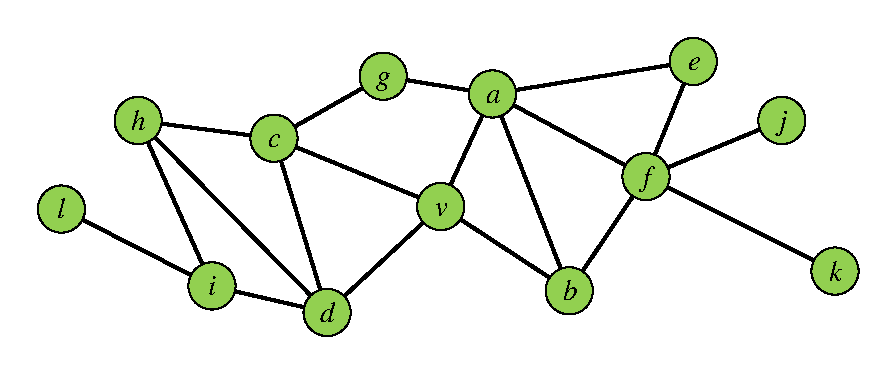
\includegraphics[width=\textwidth]{./images/figs-original.pdf}
                \caption{A given network}
                \label{fig:1-a}
        \end{subfigure}
        
        \begin{subfigure}[b]{0.38\textwidth}
                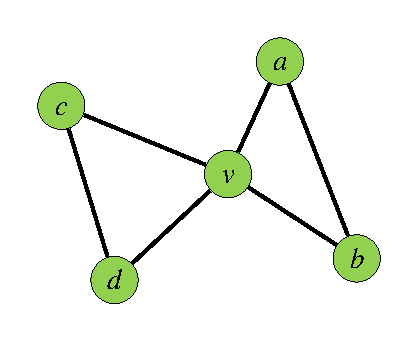
\includegraphics[width=\textwidth]{./images/ego2.pdf}
                \caption{Ego network}
                \label{fig:1-b}
        \end{subfigure}
        \begin{subfigure}[b]{0.60\textwidth}
                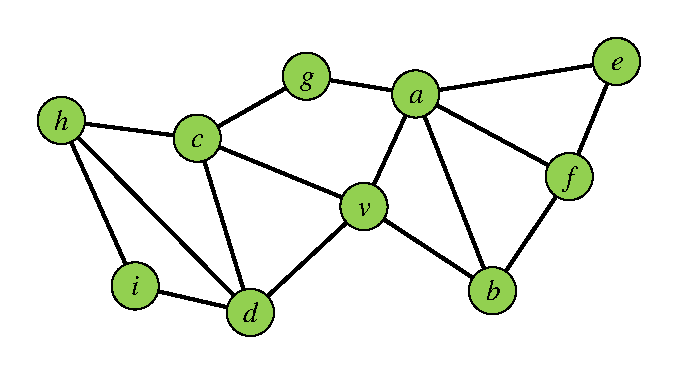
\includegraphics[width=\textwidth]{./images/second-order.pdf}
                \caption{Second-order ego network}
                \label{fig:1-c}
        \end{subfigure}
        \begin{subfigure}[b]{0.38\textwidth}
                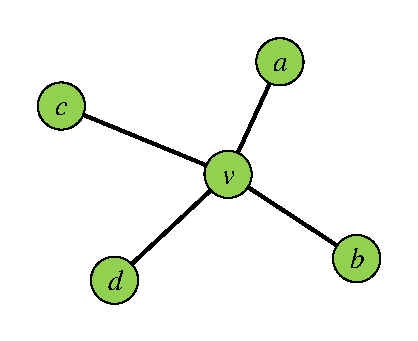
\includegraphics[width=\textwidth]{./images/friends.pdf}
                \caption{Egocentric friendship network}
                \label{fig:1-d}
        \end{subfigure}
        \begin{subfigure}[b]{0.60\textwidth}
                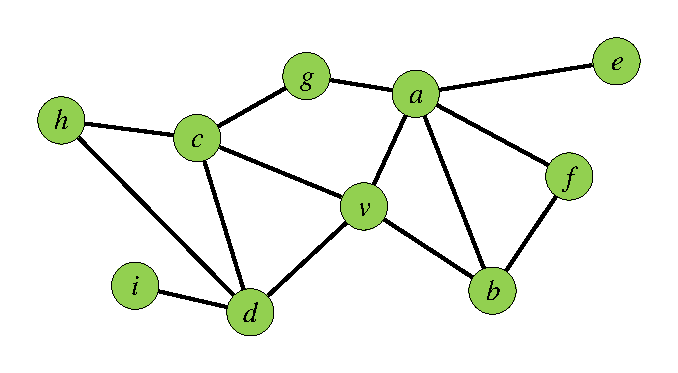
\includegraphics[width=\textwidth]{./images/multi-oder-friends.pdf}
                \caption{Second-order egocentric friendship network}
                \label{fig:1-e}
        \end{subfigure}
        \caption{The given network, and the $n$-order ego and egocentric egocentric friendship networks of vertex $v$}
        \label{fig:1}
\end{figure}

\subsection{Definitions}\label{subsec:x-egoDefinition}
In this paper, we consider a graph $G(V, E)$\footnote{We use the term {\em actors} and {\em social links} to refer to individuals, groups or organizations and their relationships in a social network. On the other hand, the graph representing a social network consists of {\em vertices} and {\em edges} representing actors and social links, respectively.} where $V$ is a set of vertices and $E$ is a set of undirected edges representing social links between vertices.
In the literature~\cite{egocentric, everett, ICCN:lbcdna, SIMBET}, given a graph $G(V, E)$ and a vertex $v \in V$, the {\em ego network} of $v$ is defined as the subgraph of $G$ consisting of $v$ and its 1-hop neighbors (i.e., vertices with an edge to $v$) as well as the edges between these vertices.
Using the notation summarized in Table~\ref{table:symbols}, this ego network can be formally extended to \emph{$n$th-order ego network} as follows:

\begin{definition}\label{def:multi-order-ego-network}
Given a graph $G(V, E)$ and a vertex $v \in V$, the \emph{$n$th-order ego network} of $v$ is defined as $\ENN{v}{n} (\LV{v}{n}, \LE{v}{n})$ where $\LV{v}{n}$ is the set of vertices whose geodesic distance from $v$ is no longer than $n$ and $\LE{v}{n}$ denotes the set of edges between the vertices in $\LV{v}{n}$.
\end{definition}

In a given graph shown at Fig.~\ref{fig:1} (a), $\LV{v}{1} = \V{v}{0} \cup \V{v}{1} = \{v, a, b, c, d\}$ and $\LE{v}{1}=\{(v, a), (v, b), (v, c), (v, d), (a, b), (c, d) \}$. The first-order ego network (i.e., just ego network) of vertex $v$, $\ENN{v}{1}(\LV{v}{1}, \LE{v}{1})$, is shown in Fig.~\ref{fig:1} (b).
Egocentric networks well model the relationships/interactions between an actor and others in a social network.
However, egocentric networks have the limitation that they do not capture a substantial amount of information if the networks are formed via a way of information diffusion.
For example, in Fig.~\ref{fig:1} (a), assume that actor $v$ received from actor $a$ the information about $a$'s 1-hop neighbors (i.e., $b$, $e$, $f$, $g$, and $v$).
Despite this information, the ego network of $v$ cannot record the social links between $a$ and $e$, between $a$ and $f$, and between $a$ and $g$ since it can represent only the social links between $v$ and each 1-hop neighbor of $v$, and between two 1-hop neighbors of $v$.
On the other hand, $n$th-order egocentric networks can hold more information than egocentric networks.
For example, the second-order ego network of vertex $v$, $\ENN{v}{2} (\LV{v}{2}, \LE{v}{2})$, is shown in Fig.~\ref{fig:1} (c).
However, it still does not contain all the linkage information of an ego's first and second-order neighbors.
For example, $f$, a second-order neighbor of $v$, has its neighbors $j$ and $k$, which does not belong to $\ENN{v}{2} (\LV{v}{2}, \LE{v}{2})$. 
If there were a way that all the neighbor information of $f$ can be delivered to $v$ via $a$ or $b$, the linkage information (e.g., $(f, j)$ and $(f, k)$) should have been used in any way. 

Egocentric friendship networks overcome the above limitation. 
Egocentric friendship network for an actor consists of the alters directly connected to the actor, along with the links between the actor and the alters. 
We extend the concept of egocentric friendship network into \emph{$n$th-order egocentric friendship network}, also called \emph{$n$th-order f-ego network}, and define it formally as follows:  
\begin{definition}\label{def:multi-order-friendship-network}
Given a graph $G(V, E)$ and a vertex $v \in V$, the \emph{$n$th-order f-ego network} of $v$ is $\FNN{v}{n}(\LV{v}{n}, \LE{v}{n} - \E{v}{n})$, where $\LV{v}{n}$ is the set of vertices that are at most $n$ hops away from $v$, $\LE{v}{n}$ is the set of edges between vertices that are at most $n$ hops away from $v$, and $\E{v}{n}$ is the set of edges between $n$-hop neighbors of $v$.
\end{definition}
Fig.~\ref{fig:1} (d) and (e) show the first-order f-ego network and the second-order f-ego network of $v$, respectively. 
$\ENN{v}{n}$ has the same vertices with $\FNN{v}{n}$, while $\FNN{v}{n}$ is different from $\ENN{v}{n}$ in that $\FNN{v}{n}$ does not contain $\E{v}{n}$. 
For example, as shown in Fig.~\ref{fig:1} (e), the second-order f-ego network of $v$ does not include the edge sets $\E{v}{2}=\{ (f, e), (h, i) \}$. It is noted that a vertex $v$ can generate its second-order f-ego network by using only neighbor information of its neighbors, along with its first-order f-ego network. 
As the same manner, for $n=1, 2, ..., n$, the $n$th-order f-ego network of an actor $v$ can be constructed with the first-order neighbor and linkage information of vertices in $V_{n-1} (v)$, along with its $(n-1)$th-order f-ego network. Formally, the $n$th-order f-ego network of a vertex $v$ is defined recursively as follows:
\begin{eqnarray}
\displaystyle
\FNN{v}{n} = 
\begin{cases}
    \displaystyle
 	\FNN{v}{n-1} + \sum_{ v_k \in V_{n-1} (v)} \FNN{v_k}{1}       & \quad \text{if } n > 1\\
    \FNN{v}{1}  & \quad \text{if } n = 1
\end{cases}
\end{eqnarray}
% The benefits of x-egocentric networks over egocentric networks are further verified in Section~\ref{evaluation}.

\subsection{Multi-order Ego and F-Ego Betweenness}\label{betweenness-sub}
% In much literature, the betweenness $C_{B}(i)$ for a node $v$ has been formally defined as follows:\begin{equation}\label{bet}
% C_{B}(v) = \frac{\sum_{s \neq v \neq t \in V, s<t}\frac{\sigma_{st}(v)}{\sigma_{st}}}{(n-1)(n-2)/2}.
% \end{equation} where $n$ is the total number of nodes, $\sigma_{st}$ is the number of shortest paths from $s$ to $t$, and $\sigma_{st}(i)$ is the number of those shortest paths that include the node $v$. In an undirected network, $\sigma_{st}=\sigma_{ts}$ and $\sigma_{st}(i)=\sigma_{ts}(i)$. The denominator denotes the total number of pairs of nodes except $v$ in an undirected network and normalizes $C_{B}(v)$ to a value between 0 and 1.
In the literature~\cite{centrality, everett, Brandes01afaster}, given a graph $G(V, E)$, the betweenness $\B{v}$ of a vertex $v$ is defined as:
\begin{equation}\label{bet}
\B{v} = \frac{\sum_{s \neq v \neq t \in V}\frac{\sigma_{st}(v)}{\sigma_{st}}}{(|V|-1)(|V|-2)}
\end{equation} where $\sigma_{st}$ is the number of shortest paths from vertex $s$ to vertex $t$ and $\sigma_{st}(v)$ is the number of those shortest paths that pass through vertex $v$. 
% \B{v} = \frac{2 \cdot \sum_{s \neq v \neq t \in V,\ s < t}\frac{\sigma_{st}(v)}{\sigma_{st}}}{(|V|-1)(|V|-2)}.
% \end{equation} where $\sigma_{st}$ is the number of shortest paths from vertex $s$ to vertex $t$ and $\sigma_{st}(v)$ is the number of those shortest paths that pass through vertex $v$. 
In the above definition, the denominator represents the total number of pairs of all vertices except $v$.
It normalizes $\B{v}$ to a value between 0 and 1.
Given an undirected graph, $\sigma_{st}=\sigma_{ts}$ and $\sigma_{st}(v)=\sigma_{ts}(v)$ for all vertices $s$, $t$, and $v$, so that it is sufficient to find either $\sigma_{st}$ or $\sigma_{ts}$ and either $\sigma_{st}(v)$ or $\sigma_{ts}(v)$.
The globally computed betweenness based on (\ref{bet}) requires much information about the whole network topology and causes large computational overheads. If the whole network were constructed via a way of information diffusion, a kind of information exchange load should be also very heavy. 
Therefore, getting local information from neighbor nodes and generating multi-order egocentric friendship networks in a distributed way are practically feasible, and calculating betweenness based on such local information is also acceptable if the betweenness is not much different from the one computed based on the global information of the whole network.
 
A node $v$'s \emph{$n$th-order ego betweenness} $\BE{n}{v}$ on its ego network $\ENN{n}{v}$ is locally computed as follows:\begin{equation}\label{ebet}
\BE{n}{v} = \frac{\sum_{s \neq v \neq t \in \V{v}{n}, s<t}\frac{\sigma_{st}^{\mathcal{E}, n}(v)}{\sigma_{st}^{\mathcal{E}, n}}}{(|\V{v}{n}|-1)(|\V{v}{n}|-2)/2} 
\end{equation} and the \emph{$n$th-order f-ego betweenness} $\BF{n}{v}$ on its f-ego network $\FNN{n}{v}$ is also locally obtained as follows: \begin{equation}\label{eebet}
\BF{n}{v} = \frac{\sum_{s \neq v \neq t \in \V{v}{n}, s<t}\frac{\sigma_{st}^{\mathcal{F}, n}(v)}{\sigma_{st}^{\mathcal{F}, n}}}{(|\V{v}{n}|-1)(|\V{v}{n}|-2)/2}
\end{equation} where $\sigma_{st}^{\mathcal{E}, n}$ and $\sigma_{st}^{\mathcal{F}, n}$ denote the number of shortest paths from vertex $s$ to vertex $t$ in $\ENN{v}{n}$ and $\FNN{v}{n}$, while $\sigma_{st}^{\mathcal{E}, n}(v)$ and $\sigma_{st}^{\mathcal{F}, n}(v)$ denote the number of shortest paths from vertex $s$ to vertex $t$ through vertex $v$ in $\ENN{v}{n}$ and $\FNN{v}{n}$. 

In this paper, we consider the situations where each node computes its betweenness using either its $n$th-order ego network or $n$th-order f-ego network, and then uses the result as an estimate of its true betweenness in the entire network.

% To compare the accuracy of $\BE{n}{v}$ or $\BX{v}$, we first use the Spearman's rank correlation which measures the {\em monotonic} relationship between the ranked variables of $\BX{v}$ and $\B{v}$ or $\BE{n}{v}$ and $\B{v}$.  The correlation value can vary between -1.0 and +1.0. The closer value is to +1.0, the stronger the association between the values. For the sake of completeness, we also measure the well-known Pearson correlation. The Pearson correlation coefficient assesses a {\em linear} relationship between the two variables and the calculation is based not on the ranked variables, but on the actual betweenness values.
% For the networks shown in Fig. \ref{}, Table \ref{comparison} shows the comparison of globally computed, ego, and x-ego betweenness. Although the actual betweenness values are different with each other, we can see that 1) the rank order of the three betweenness values are very similar to each other, and 2) the rank order of x-ego betweenness is more similar to the one of globally computed betweenness than the one of ego betweenness. We will verify the details with real mobility trace data in Section IV.

\begin{center}
\begin{table*}[t]
 \caption{Comparison of betweenness, first-order ego betweenness, and first-order f-ego betweenness for the graph shown in Fig. \ref{eego} (a), (b), and (d) (the Pearson correlation is 0.63 between $\B{v}$ and $\BE{n}{v}$ and 0.90 between $\B{v}$ and $\BF{n}{v}$, and the Spearman correlation is 0.79 between $\B{v}$ and $\BE{n}{v}$ and 0.93 between $\B{v}$ and $\BF{n}{v}$)}\label{comparison}
 \resizebox{13.7cm}{!} {
 \begin{tabular}{|c|c|c|c|c|c|c|c|c|c|c|c|c|c|c|}
 \hline
\multicolumn{2}{|c|}{Nodes} & v & a & b & c & d & e & f & g & h & i & j & k & l \\
 \hline
\multirow{2}{*}{$\B{v}$} & Value & 0.405 & 0.383 & 0.124 & 0.131 & 0.286 & 0.000 & 0.318 & 0.049 & 0.030 & 0.167 & 0.000 & 0.000 & 0.000\\
\hhline{~--------------}
& Rank & 1 & 2 & 7 & 6 & 4 & 10 & 3 & 8 & 9 & 5 & 10 & 10 & 10\\
\hhline{---------------}
\multirow{2}{*}{$\BE{n}{v}$} & Value & 0.667 & 0.750 & 0.167 & 0.583 & 0.333 & 0.000 & 0.833 & 1.000 & 0.167 & 0.667 & 0.000 & 0.000 & 0.000\\
\hhline{~--------------}
& Rank & 4 & 3 & 8 & 6 & 7 & 10 & 2 & 1 & 8 & 4 & 10 & 10 & 10\\
\hhline{---------------}
\multirow{2}{*}{$\BF{n}{v}$} & Value & 0.383 & 0.500 & 0.125 & 0.269 & 0.339 & 0.000 & 0.524 & 0.214 & 0.133 & 0.400 & 0.000 & 0.000 & 0.000\\
\hhline{~--------------}
& Rank & 4 & 2 & 9 & 6 & 5 & 10 & 1 & 7 & 8 & 3 & 10 & 10 & 10\\
\hhline{---------------}
 \hline
 \end{tabular}
}
\end{table*}
\end{center}

Table~\ref{comparison} shows, for every vertex $v$ in Fig.~\ref{eego}, the betweenness ($\B{v}$), ego betweenness ($\BE{n}{v}$), and x-ego betweenness ($\BF{n}{v}$).
In this table, for most of the vertices, x-ego betweenness is closer to betweenness than ego-betweenness mainly because it is derived from a larger number of vertices and edges.
For this reason, the correlation coefficient (also known as the Pearson correlation coefficient) of x-ego betweenness and betweenness (0.9) is higher than that of ego-betweenness and betweenness (0.63).
The advantage of x-ego betweenness over ego betweenness can also be observed in terms of Spearman's rank correlation, which indicates, given two series $\mathcal{X}=(X_1, X_2, \cdots, X_N)$ and $\mathcal{Y}=(Y_1, Y_2, \cdots, Y_N)$, the correlation between $(r_{\mathcal{X}}(X_1), r_{\mathcal{X}}(X_2)$ $, \cdots, r_{\mathcal{X}}(X_N))$ and $(r_{\mathcal{Y}}(Y_1), r_{\mathcal{Y}}(Y_2), \cdots, r_{\mathcal{Y}}(Y_N))$, where $r_{\mathcal{X}}(X_i)$ and $r_{\mathcal{Y}}(Y_i)$ represent the rank of $X_i$ in $\mathcal{X}$ and that of $Y_i$ in $\mathcal{Y}$, respectively.
In Table~\ref{comparison}, Spearman's correlation is 0.93 between x-ego betweenness and betweenness and 0.79 between ego betweenness and betweenness.
In Section~\ref{evaluation}, we further demonstrate the benefit of x-ego betweenness using wireless trace data.

\subsection{Properties of Multi-order Egocentric Friendship Networks}\label{mfn_properties}
In this section, we present four properties of multi-order egocentric egocentric friendship networks. 
These properties enable efficient multi-order betweenness computation (Section~\ref{computation}). 
As in Brandes' work~\cite{Brandes01afaster}, we denote the \emph{dependency} of vertices $s$ and $t$ on vertex $v$ as $\D{s}{t}{v} = \frac{\sigma_{st}(v)}{\sigma_{st}}$.
Then, the betweenness of $v$ (Equation (\ref{bet})) can be computed by adding the dependency values for all pairs of vertices excluding $v$.
To quickly calculate such dependency values in multi-order egocentric egocentric friendship networks, we have identified the properties explained below. 
% By Equation (\ref{bet}), we can know that the betweenness of $v$ can be obtained by summing the dependencies for all pairs of vertices, except for $v$, in $\XN{v}$.
% % The exhaustive search of such all shortest paths is computationally expensive. 
% We identify the following properties, {\em Theorem \ref{theorem1}, \ref{theorem2}, \ref{theorem3}}, and  {\em \ref{theorem4}}, to obtain such dependencies with low computational overhead.
% % Therefore, we need to devise {\em skip conditions} or (\ldots) to reduce the computational burden.  
\begin{theorem}
\label{theorem1} 
Assume a vertex $v$, its x-ego network $\XN{v}$, and its two different 1-hop neighbors $s$ and $t$ (i.e., $s, t \in \V{v}{1}$ and $s \ne t$).
Then, $\D{s}{t}{v} = 0$ if there is an edge between $s$ and $t$ (i.e., $\{s, t\} \in \E{v}{1}$).
\begin{proof}
Since $\{s, t\} \in \E{v}{1}$, $d(s, t) = 1$.
Furthermore, $s, t \in \V{v}{1}$, meaning that $d(s, v) + d(v, t) = 1 + 1 = 2 > d(s, t) = 1$ (i.e., no shortest path from $s$ to $t$ passes through $v$).
Therefore, $\D{s}{t}{v} = \sigma_{st}(v)/\sigma_{st} = 0/\sigma_{st} = 0$.\hfill\qed
\end{proof}
\end{theorem}
\begin{example}
In Fig.~\ref{eego2}(b), $\D{a}{b}{v} = 0$ since $a, b \in \V{v}{1}$ and there is an edge between $a$ and $b$.
\end{example}
% Theorem \ref{theorem1} will take on a key role as a computation skipping rule in the algorithm to compute the x-ego betweenness, $\BX{v}$. In particular, it will reduce the computational overload substantially when a vertex $v$'s x-ego network exhibits a strong community structure (i.e., nodes in egocentric networks tend to interact with each other). Since friends of a friend are likely to be friends as well, we can expect that this transitivity should be frequently observed in x-egocentric networks derived by a DTN. 
% 
% In case that the skipping rule presented by Theorem \ref{theorem1} cannot be applied for a pair of $v$'s two 1-hop neighbors, the dependency of them is computed by using the following Theorem \ref{theorem2}. 
Theorem \ref{theorem1} allows us to quickly compute dependencies particularly when x-egocentric networks exhibit a strong community structure (i.e., 1-hop neighbors of a node tend to have direct social links between them).
In Section~\ref{evaluation}, we show this benefit using wireless trace data.
When Theorem \ref{theorem1} cannot be applied to $v$'s 1-hop neighbors $s$ and $t$ (i.e., there is no edge between $s$ and $t$), the dependency of $s$ and $t$ on $v$ can be computed using the following theorem.
\begin{theorem}
\label{theorem2} 
Assume a vertex $v$, its x-ego network $\XN{v}$, and its two different 1-hop neighbors $s$ and $t$ (i.e., $s, t \in \V{v}{1}$ and $s \ne t$).
Then, $\D{s}{t}{v} = {1}/{|\V{s}{1} \cap \V{t}{1}|}$ if there is no edge between $s$ and $t$ (i.e., $\{s, t\} \notin \E{v}{1}$).
\begin{proof}
Since $\{s, t\} \notin \E{v}{1}$, $d(s, t) > 1$.
In this case, $d(s, t) = 2$ due to the path $s - v - t$.
Furthermore, (i) the number of shortest paths from $s$ to $t$ (i.e., paths whose length is 2) can be expressed as $\sigma_{st} = |\V{s}{1} \cap \V{t}{1}|$.
%  indicates the number of shortest paths starting from $v_s \in N_0$ and terminating at $v_t \in N_0$.
On the other hand, (ii) the path $s-v-t$ is the only shortest path from $s$ to $t$ that passes through $v$ (i.e., $\sigma_{st}(v) = 1$) since the length of that path is 2, which must be smaller than the length of any other path from $s$ to $t$ that passes through $v$.
By (i) and (ii), $\D{s}{t}{v} = \sigma_{st}(v)/\sigma_{st} = {1}/{|\V{s}{1} \cap \V{t}{1}|}$.\hfill\qed
\end{proof}
\end{theorem}
% \begin{equation}
% \D{s}{t}{v} =
%   \begin{cases}
%    0       & \text{if $(s, t) \in E$} \\
%    {\displaystyle \frac {1}{|\V{s}{1} \cap \V{t}{1}|}} & \text{ otherwise.} \\
%   \end{cases}
% \end{equation}
\begin{example}
\label{example2} 
In Fig.~\ref{eego2}(b), vertices $a$ and $c$ are 1-hop neighbors of $v$ and there is no edge between $a$ and $c$.
Furthermore, $\V{a}{1} = \lbrace b, e, f, g, v\rbrace$ and $\V{c}{1} = \lbrace d, g, h, v\rbrace$.
Therefore, $\D{a}{c}{v}=1/|\V{a}{1} \cap \V{c}{1}|=1/|\{g, v \}|=1/2$.
% $\LV{a}{1} = \lbrace v, b, e, f, g\rbrace$, $\LV{c}{1} = \lbrace v, d, g, h\rbrace$ and $\LV{d}{1} = \lbrace v, c, h, i\rbrace$. So, node $v$ can get the non-zero $\D{a}{c}{v}=1/2=0.5$ and $\D{a}{d}{v}=1/1=1$ because $v$ knows that $a$ does not share any edge with $c$ and $d$, $|\LV{a}{1} \cap \LV{c}{1}| = |\lbrace v, g\rbrace|=2$, and $|\LV{a}{1} \cap \LV{d}{1}| = |\lbrace v\rbrace$| = 1. 
\end{example}
Just like Theorem~\ref{theorem1}, the following theorem quickly computes the dependency of two vertices on a vertex $v$.
While the former applies to a pair of 1-hop neighbors of $v$, the latter applies to a pair of a 1-hop or 2-hop neighbor and a 2 hop-neighbor of $v$.
% The following Theorem \ref{theorem3} presents another skipping rule to reduce the computation overload of the dependency for an 1 or 2-hop neighbor and a 2-hop neighbor of $v$.
\begin{theorem}
\label{theorem3} 
Assume a vertex $v$, its x-ego network $\XN{v}$, a vertex $s \in \LV{v}{2}$, and another vertex $t \in \V{v}{2}$ such that $s \ne t$.
Then, $\D{s}{t}{v} = 0$ if $\D{s}{n}{v} = 0$ for a 1-hop neighbor vertex $n$ of vertex $t$ (i.e., for $n \in \V{t}{1}$).
\begin{proof}
Since $\D{s}{n}{v} = 0$ (i.e., no shortest path from $s$ to $n$ passes through $v$), (i) $d(s, n) < d(s, v) +d(v, n)$.
Then, (ii) $d(s, t) \le d(s, n) + d(n, t) < d(s, v) + d(v, n) + d(n, t)$ by (i).
Furthermore, $n \in \V{t}{1}$ and $t \in \V{v}{2}$, meaning that vertex $n$ is either a 1-hop or a 3-hop neighbor of $v$.
In $\XN{v}$, however, any vertex including $n$ is at most 2 hops away from $v$.
For this reason, $n$ is a 1-hop neighbor of $v$.
Since $d(v, n)$=$d(n, t)$=$1$ and $d(v, t)=2$, (iii) $d(v, n) + d(n, t) = d(v, t)$. 
By (ii) and (iii), $d(s, t) < d(s, v) +d(v, t)$ (i.e., no shortest path from $s$ to $t$ passes through $v$).
Therefore, $\D{s}{t}{v}  = \sigma_{st}(v)/\sigma_{st} = 0/\sigma_{st} = 0$.\hfill\qed
\end{proof}
\end{theorem}
\begin{example}
In Fig. \ref{eego2}(b), $b \in \LV{v}{2}$ and $g \in \V{v}{2}$. 
Furthermore, for a 1-hop neighbor $a$ of $g$, $\D{b}{a}{v}=0$ (Theorem \ref{theorem1}).
Therefore, by Theorem \ref{theorem3}, $\D{b}{g}{v}=0$.
\end{example}
Given vertices $s \in \LV{v}{2}$ and $t \in \V{v}{2}$ such that $s \ne t$, Theorem~\ref{theorem3} cannot be applied if $\D{s}{n}{v} > 0$ for every 1-hop neighbor $n$ of $t$.
In this case, the dependency of $s$ and $t$ on $v$ can be obtained using the following theorem.
% Lastly, the following Theorem \ref{theorem4} presents that the harmonic mean can be used to compute the dependency for an 1 or 2-hop neighbor and a 2-hop neighbor of $v$, if they do not satisfy the condition of Theorem \ref{theorem3}. 
\begin{theorem}
\label{theorem4} 
Assume a vertex $v$, its x-ego network $\XN{v}$, a vertex $s \in \LV{v}{2}$, and another vertex $t \in \V{v}{2}$ such that $s \ne t$.
Then, $\D{s}{t}{v} = \bar{H}(\{\D{s}{n}{v} : n \in \V{t}{1}\})$ if $\D{s}{n}{v} > 0$ for every 1-hop neighbor $n$ of vertex $t$, where $\bar{H}(\{\D{s}{n}{v} : n \in \V{t}{1}\})$ denotes the {\em harmonic mean} computed over $\{\D{s}{n}{v} : n \in \V{t}{1}\}$.
\begin{proof}
We prove this theorem considering the following two cases.
% in two cases, $s \in \LV{v}{1}$ or $s \in \LV{v}{2}-\LV{v}{1}$, separately:
\noindent [Case I. $s$ is a 1-hop neighbor of $v$ (i.e., $s \in \V{v}{1}$)]
% Let us assume there are $m$ 1-hop neighbors of $t$ in $\XN{v}$ and let $n_i$ denote the $i$th 1-hop neighbor of $t$ such that $\D{s}{n_i}{v} > 0$. In $\XN{v}$, each $n_i$ is also an 1-hop neighbor of $v$ (i.e., $n_i \in \LV{v}{1}$) and $\D{s}{n_i}{v} = {1}/{|\LV{s}{1} \cap \LV{n_i}{1}|}$ by Theorem \ref{theorem2}. 
% Furthermore, (i) $|\LV{s}{1} \cap \LV{n_i}{1}|=1/\D{s}{n_i}{v}$ represents the number of shortest paths from $s$ to $n_i$ (i.e., $\sigma_{sn_i}$) and the total number of shortest paths from $s$ to $t$ can be expressed as $\sigma_{st} = \sum_{i=1}^m 1/\D{s}{n_i}{v}$ since each $n_i$ shares an edge with $t$. On the other hand, (ii) the path $s-v-n_i-t$ is the only shortest path from $s$ to $t$ via both $v$ and $n_i$ since the length of the path is 3 and any other path from $s$ to $t$ via both $v$ and $n_i$ must be longer. It means that there are $m$ shortest paths from $s$ to $t$ via $v$ (i.e., $\sigma_{st}(v)=m$). By (i) and (ii), $\D{s}{t}{v} = \frac{m}{\sum_{i=1}^m 1/\D{s}{n_i}{v}} = \bar{H}(\D{s}{n}{v})$.
Let $n_i$ ($i=1,2,\cdots, m$) denote the $i$th 1-hop neighbor of $t$.
Then, each $n_i$ is a 1-hop neighbor of $v$ since, in $\XN{v}$, any 2-hop neighbor (including $t$) of $v$ can be connected only to a 1-hop neighbor of $v$ (Definition~\ref{def:xego-network}).
Thus, by Theorem \ref{theorem2}, $\D{s}{n_i}{v} = {1}/{|\V{s}{1} \cap \V{n_i}{1}|}$. 
Since $|\V{s}{1} \cap \V{n_i}{1}|$ represents the number of shortest paths from $s$ to $n_i$ (i.e., $\sigma_{sn_i}$) and each $n_i$ has an edge to $t$, the total number of shortest paths from $s$ to $t$ can be expressed as (i) $\sigma_{st} = \sum_{i=1}^m |\V{s}{1} \cap \V{n_i}{1}| = \sum_{i=1}^m 1/\D{s}{n_i}{v}$. 
On the other hand, the path $s-v-n_i-t$ is the only shortest path from $s$ to $t$ via both $v$ and $n_i$ since the length of the path is 3 and any other path from $s$ to $t$ via both $v$ and $n_i$ must be longer.
For this reason, (ii) there are $m$ shortest paths from $s$ to $t$ via $v$ (i.e., $\sigma_{st}(v)=m$).
By (i) and (ii), $\D{s}{t}{v} = \frac{m}{\sum_{i=1}^m 1/\D{s}{n_i}{v}} = \bar{H}(\D{s}{n}{v})$.
\noindent [Case II. $s$ is a 2-hop neighbor of $v$ (i.e., $s \in \V{v}{2}$)]
Let $n_i~(i=1,2,\cdots,m)$ denote the $i$th 1-hop neighbor of $t$. 
Let also $p_j~(j=1,2,\cdots,k)$ denote the $j$th 1-hop neighbor of $s$.
In $\XN{v}$, 2-hop neighbors (including $s$ and $t$) of $v$ can be connected only to a 1-hop neighbor of $v$.
For this reason, any shortest path from $s$ to $t$ must contain a shortest path from $p_j$ to $n_i$ for some $j$ and $i$ 
% Since $n_i$ and $p_j$ respectively shares an edge with $t$ and $s$, the shortest path from $n_i$ to $n_j$ for a pair of $i$ and $j$ always corresponds to the one from $s$ to $t$ 
(i.e., $\sigma_{st} = \sum_{i=1}^m \sum_{j=1}^k |\V{n_i}{1} \cap \V{p_j}{1}|$). 
For a pair of $i$ and $j$, on the other hand, the path $n_i-v-p_j$ is the only shortest path from $n_i$ to $p_j$ via $v$ and so is the path $t-n_i-v-p_j-s$ (i.e., $\sigma_{st}(v)=mk$). 
Therefore, 
\begin{eqnarray}
\D{s}{t}{v} 
&=& \frac{mk}{\sum_{i=1}^m \sum_{j=1}^k |\V{n_i}{1} \cap \V{p_j}{1}|} \nonumber \\ 
&=& \frac{mk}{\sum_{i=1}^m \sum_{j=1}^k 1/\D{n_i}{p_j}{v}} \nonumber \\ 
&=& \frac{m}{\sum_{i=1}^m \frac {\sum_{j=1}^k 1/\D{n_i}{p_j}{v}}{k}} \nonumber \\ 
&=& \frac{m}{\sum_{i=1}^m 1/\D{n_i}{s}{v}} \nonumber \\ 
&=& \frac{m}{\sum_{i=1}^m 1/\D{s}{n_i}{v}} \nonumber  \\
&=& \bar{H}(\D{s}{n}{v}).   \nonumber
\end{eqnarray}
\label{harmonic_eq}
\end{proof}
\end{theorem}
% \label{harmonic} 
% For a vertex $v$, its x-ego network $\XN{v}$, a vertex $s \in \V{v}{1} \cup \V{v}{2}$ and another vertex $t \in \V{v}{2}$, let $n_1, n_2, \cdots, n_i$ ($n_i \leq u$) denote the 1-hop neighbor vertices of vertex $t$. 
% Then, 
% \begin{equation}
% \D{s}{t}{v} =
%   \begin{cases}
%    0      &\text{if $\exists k, \D{s}{n_k}{v} = 0$} \\
%    \bar H (\D{s}{n_k}{v}) &\text{otherwise.}
%    \end{cases}
% \end{equation} where $\bar H_{st}$ is the harmonic mean for all the non-zero $f_{s{n_k}}$ values.
% \end{theorem}
% \begin{proof}
% ...\\
% ...\\
% ...\\
% ... \qed
% \end{proof}
\begin{example}
In Fig.~\ref{eego2}(b), % consider the dependency $\D{a}{h}{v}$ of $a \in \LV{v}{2}$ and $h \in \V{v}{2}$ on $v$. In this example, 
$\V{h}{1} = \{c,d\}$.
By Theorem \ref{theorem2}, $\D{a}{c}{v}=\frac{1}{2}$ and $\D{a}{d}{v}=1$.
Therefore, by Theorem \ref{theorem4}, $\D{a}{h}{v}\!=\!\bar{H}(\{\D{a}{n}{v} : n \in \V{h}{1}\})\!=\!\bar{H}(\{\D{a}{c}{v},\D{a}{d}{v}\})\!=\!\frac{2}{\frac{1}{\frac{1}{2}} + \frac{1}{1}}=\frac{2}{3}$.  
% For each 1-hop neighbor $n$ of $h$ (i.e., $n \in \V{h}{1} = \{ c,d\}$,  and from Theorem \ref{theorem2} it also knows $\D{a}{c}{v}=1/2$ and $\D{a}{d}{v}=1/1$ for $h$'s two 1-hop neighbors, $c$ and $d$. Therefore, we can get $\D{a}{h}{v}$=$\bar{H}(\D{a}{c}{v},\D{a}{d}{v})$=$2/3$. 
% Similarly, $\D{c}{e}{v}=\bar{H}(\D{c}{a}{v})=1/2$ where $c \in \LV{v}{1} (\subset \LV{v}{2})$ and $e \in \LV{v}{2}-\LV{v}{1}$, since $\LV{e}{1}=\{e,a\}$, $\D{c}{a}{v}=1/2$ and $\bar{H}(\D{c}{a}{v})=\D{c}{a}{v}$.
\end{example}
% These four properties will be used in the algorithm proposed in Section \ref{computation} to compute the x-ego betweenness of a DTN node.

\section{Betweenness in Multi-order Friendship Networks}\label{sec:betweenness}
In this section, we propose a new algorithm to calculate the betweenness centrality in the multi-oder friendship
networks.


\section{Evaluation}
\label{evaluation}

\section{EEGO}
\label{eego}

\section{Computation}
\label{computation}


%% The Appendices part is started with the command \appendix;
%% appendix sections are then done as normal sections
%% \appendix

%% \section{}
%% \label{}

%% If you have bibdatabase file and want bibtex to generate the
%% bibitems, please use
%%
\bibliographystyle{elsarticle-num-names}
\bibliography{../../LinkPaper}

%% else use the following coding to input the bibitems directly in the
%% TeX file.

%\begin{thebibliography}{00}

%% \bibitem[Author(year)]{label}
%% Text of bibliographic item

%\bibitem[ ()]{}

%\end{thebibliography}
\end{document}

\endinput
%%
%% End of file `elsarticle-template-harv.tex'.
